% ===========================================================================
\section{A assinatura de um par}\label{sec:assinatura}
% ===========================================================================

A última imagem é a de escala mais fina: não um bloco, mas um único par de
inteiros vizinhos. Ela mostra que a presença de um único tom é detectável, e a
que preço.

\subsection{O coeficiente em uma frequência}

Seja $N\ge2$ e considere o sinal dos primos até $N$,
\begin{equation}\label{eq:Rprimo}
  R(t) \;=\; -\sum_{\substack{p\le N\\ p\ \mathrm{primo}}}
  \frac{\cos\bigl(t\,\nfreq p\bigr)}{\sqrt p},
\end{equation}
que é a soma das componentes fundamentais \eqref{eq:serie}, com amplitude
$p^{-1/2}$, para os primos. Para $q\ge5$ defina
\[
  \hat a_q \;=\;
  \frac{\bigl|\hat R(\freq q)\bigr|}{T/(2\sqrt q)},
  \qquad
  \hat R(f) \;=\; \int_0^T R(t)\,e^{-2\pi i f t}\,dt ,
\]
isto é, a amplitude medida em $\freq q$ normalizada pela amplitude que um único
tom de tamanho $q$ produziria.

\begin{proposicao}\label{prop:gemeo}
Seja $q\ge5$ e defina
\[
  \varepsilon_q \;=\;
  \frac{2\sqrt q}{T}\sum_{\substack{p\le N\\ p\neq q}}
  \frac{1}{\sqrt p\,\bigl|\nfreq p-\nfreq q\bigr|}.
\]
Então
\[
  \bigl|\hat a_q - \mathbf 1_{q\in\mathcal P}\bigr| \;\le\; \varepsilon_q ,
\]
onde $\mathbf 1_{q\in\mathcal P}$ vale $1$ se $q$ é primo e $q\le N$, e $0$ caso
contrário. Além disso existem constantes absolutas $0<c<C$ com
\[
  \varepsilon_q \;\le\; C\,\frac{q\log q}{T},
  \qquad\text{e}\qquad
  \varepsilon_q \;\ge\; c\,\frac{q}{T}
  \ \text{ se } q-2 \text{ é primo}.
\]
\end{proposicao}

\begin{proof}
Escreva $\hat R=\sum_p \hat S_p$ com
$\hat S_p=-\frac{1}{2\sqrt p}\bigl[F(\nu_p-\nu_q)+F(-\nu_p-\nu_q)\bigr]$ e
$F(\alpha)=\bigl(e^{i\alpha T}-1\bigr)/(i\alpha)$, de modo que
$|F(\alpha)|\le 2/|\alpha|$ para $\alpha\neq0$ e $F(0)=T$.

\emph{Termo próprio.} Se $q\in\mathcal P$ então
$\hat S_q=-\tfrac{T}{2\sqrt q}\bigl(1+O((T\nu_q)^{-1})\bigr)$, e a normalização por
$T/(2\sqrt q)$ dá $1+O((T\nu_q)^{-1})$.

\emph{Termos alheios.} Para $p\neq q$,
\[
  \bigl|\hat S_p\bigr| \;\le\;
  \frac{1}{2\sqrt p}\Bigl(\frac{2}{|\nu_p-\nu_q|}+\frac{2}{\nu_p+\nu_q}\Bigr)
  \;\le\; \frac{1}{\sqrt p\,\bigl|\nfreq p-\nfreq q\bigr|}\,(1+\eta_p),
\]
com $\eta_p=O((T\nu_p)^{-1})$. Dividindo por $T/(2\sqrt q)$ obtém-se a soma que
define $\varepsilon_q$.

\emph{Cota superior.} Para $p$ com $|p-q|<q/2$, use
$|\nfreq p-\nfreq q|\ge |p-q|/\max(p,q)\ge |p-q|/(2q)$; então
\[
  \sum_{|p-q|<q/2}\frac{1}{\sqrt p\,\bigl|\nfreq p-\nfreq q\bigr|}
  \;\le\; \frac{2q}{\sqrt q}\sum_{p\neq q}\frac{1}{|p-q|}
  \;=\; O\bigl(\sqrt q\log q\bigr).
\]
Para $|p-q|\ge q/2$ tem-se $|\nfreq p-\nfreq q|\ge\log(3/2)$, e a soma restante é
$O\bigl(\sqrt q/\log q\bigr)$, já que $\sum_{p\le N}p^{-1/2}=O(\sqrt N/\log N)$ e
$N\asymp q$. Multiplicando por $2\sqrt q/T$ resulta $\varepsilon_q=O(q\log q/T)$.

\emph{Cota inferior.} Se $q-2$ é primo, o termo $p=q-2$ tem
$|\nfreq p-\nfreq q|=\log(1+2/(q-2))\le 2/(q-2)$, logo contribui com pelo menos
\[
  \frac{2\sqrt q}{T}\cdot\frac{1}{\sqrt q}\cdot\frac{q-2}{2}\;\ge\;\frac{q}{2T},
\]
independentemente de $T$.
\end{proof}

O conteúdo é o esperado do dicionário: a presença do tom é legível como uma
amplitude de ordem $1$; a ausência deixa apenas o vazamento dos tons vizinhos,
cuja amplitude relativa é da ordem de $q/T$. O parâmetro que governa a leitura é,
portanto, a razão $T/q$. A cota superior carrega um fator $\log q$ perdido na
estimativa grosseira da soma, mas a cota inferior mostra que a ordem correta é
$q/T$: o vizinho $q-2$ contribui sempre com essa ordem.

\subsection{O contraste}

A Proposição~\ref{prop:gemeo} dá o contraste entre os dois casos:
\[
  \frac{\text{sinal}}{\text{fundo}} \;\asymp\; \frac{1}{q/T} \;=\; \frac{T}{q}.
\]
Aumentar a janela aumenta o contraste linearmente, o que é o análogo, no nível
local, da lei de escala do Teorema~\ref{teo:custo}: para separar um tom do fundo
produzido pelos vizinhos, é preciso uma janela que cresça com o próprio $q$.

\subsection{Gêmeos e mistos}

A aplicação natural é a comparação de pares. Para cada primo $p\le N-2$, o par
$(p,p+2)$ é \emph{gêmeo} se $p+2$ é primo, e \emph{misto} caso contrário. A
Proposição~\ref{prop:gemeo} diz, sem mais hipóteses, que $\hat a_{p+2}\approx1$ no
primeiro caso e $\hat a_{p+2}\approx0$ no segundo, com folga da ordem de
$T/(p+2)$.

A Figura~\ref{fig:gemeos} mostra as duas distribuições para $N=300$ e
$T=6500$, medidas com o coeficiente exato (sem grade, isto é, avaliando a integral
\eqref{eq:Rprimo} diretamente na frequência). Os gêmeos se acumulam perto de $1$,
os mistos perto de $0$, e não há sobreposição.

\begin{figure}[htbp]
\centering
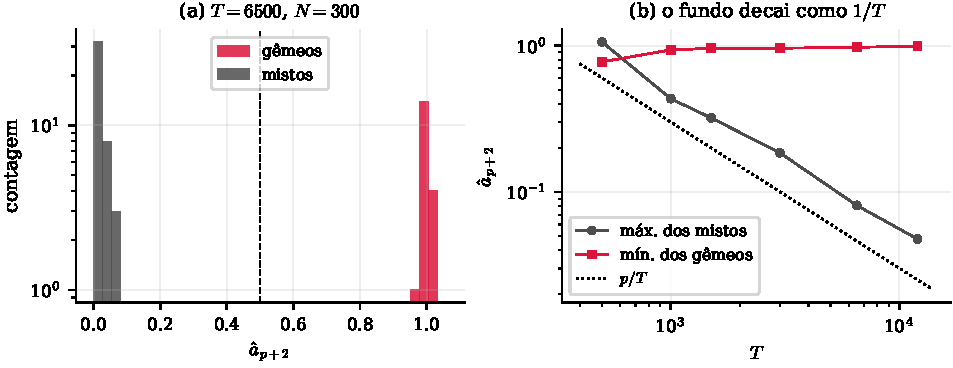
\includegraphics[width=0.95\textwidth]{figuras/f6_gemeos.pdf}
\caption{(a) Distribuição de $\hat a_{p+2}$ para os $62$ pares $(p,p+2)$ com
$p\le299$, com $T=6500$. (b) O máximo entre os mistos e o mínimo entre os gêmeos
em função de $T$; o fundo decai como $p/T$, como prevê a
Proposição~\ref{prop:gemeo}.}
\label{fig:gemeos}
\end{figure}

\begin{table}[htbp]
\centering
\small
\begin{tabular}{rrrr}
\toprule
$T$ & $\max$ dos mistos & $\min$ dos gêmeos & separação \\
\midrule
$500$   & $1{,}058$ & $0{,}774$ & falha \\
$1\,000$& $0{,}434$ & $0{,}934$ & completa \\
$1\,500$& $0{,}321$ & $0{,}958$ & completa \\
$3\,000$& $0{,}185$ & $0{,}959$ & completa \\
$6\,500$& $0{,}081$ & $0{,}973$ & completa \\
$12\,000$& $0{,}048$& $0{,}991$ & completa \\
\bottomrule
\end{tabular}
\caption{O fundo cai como $1/T$ e a separação se completa quando $T$ ultrapassa
algumas vezes $p_{\max}=299$.}
\label{tab:gemeos}
\end{table}

A assinatura é local: ela não usa a posição dos primos na reta, apenas a presença
ou ausência de um tom na frequência do par. É a instância mais fina do Teorema
\ref{teo:irred}: a irredutibilidade de $p+2$, traduzida em presença de frequência,
é legível para quem pode pagar a janela.

\subsection{Uma nota sobre a leitura}

Duas armadilhas práticas, ambas consequência da Proposição~\ref{prop:janela},
merecem registro porque afetam qualquer medição deste tipo.

A primeira é a grade. Se o coeficiente é avaliado em uma transformada discreta, a
frequência $\freq q$ raramente coincide com uma célula da grade, e o máximo lido
pode ser até $\operatorname{sinc}(\pi/2)\approx0{,}64$ do valor real. A correção é
avaliar o coeficiente na frequência exata, ou usar uma janela de afunilamento e
corrigir o ganho coerente.

A segunda é a faixa de leitura. Se a busca do pico varre $\pm W$ células e esse
intervalo inclui o pico do vizinho $q-2$, a leitura de um par misto herda a altura
do pico alheio — e a separação desaparece, como mostra a
Tabela~\ref{tab:janela}. Nenhum aumento de $T$ conserta isso: com $W$ fixo, a
condição $2W+1<T/(\pi q)$ é respeitada ou não.

Essas duas observações não são detalhes de implementação; são parte do conteúdo
matemático da representação, porque dizem em que condições a leitura de um
coeficiente corresponde ao termo que se quer medir.
